\documentclass{article}
\usepackage{fullpage}
\usepackage{graphicx}
\usepackage[spanish]{babel}
\usepackage{amssymb}
\usepackage{amsmath}
\usepackage{cancel}
\usepackage{minted}
\usepackage{caption}
\usepackage{array}
\usepackage[linesnumbered,ruled,lined]{algorithm2e}
\DontPrintSemicolon
\SetKwRepeat{Do}{do}{while}


%%%%% Comandos Personalizados %%%%%
\newcommand{\N}{\mathbb{N}}
\newcommand{\R}{\mathbb{R}}
\newcommand{\Q}{\mathbb{Q}}
\newcommand{\E}{\mathbb{E}}
\newcommand{\PP}{\mathbb{P}}
\newcommand{\la}{\leftarrow}
\newcommand{\ra}{\rightarrow}
\newcommand{\lra}{\leftrightarrow}
\newcommand{\Ra}{\Rightarrow}
\newcommand{\La}{\Leftarrow}
\newcommand{\LRa}{\Leftrightarrow}
\newcommand{\sub}{\subseteq}
\newcommand{\matro}{\mathcal{M}}

\newcommand{\twopartdef}[4]
{
	\left\{
		\begin{array}{ll}
			#1 &  \text{#2} \\
			#3 &  \text{#4}
		\end{array}
	\right.
}

%%%%%  Fin Comandos Personalizados %%%%%


     %%%%%%%%%% MODIFICAR %%%%%%%%%%
\newcommand{\alumnos}{Benja Sanchez, Victor Ruiz}
\newcommand{\departamento}{Departamento de Ingenieria Industrial y de Sistemas}
\newcommand{\ramo}{Optimización}
\newcommand{\sigla}{ICS1113}
\newcommand{\titulo}{Tarea 1}
\newcommand{\semestre}{01 }
\newcommand{\anio}{2023}
\newcommand{\med}{\frac{1}{2}}
\newcommand{\indep}{\mathcal{I}}
     %%%%%%%%%% FIN MODIFICAR %%%%%%%%%%



\renewcommand{\thesubsection}{\alph{subsection}}

\begin{document}

\thispagestyle{empty}

\begin{minipage}{2cm}
\vspace{-1.5cm}

\includegraphics[width=2cm]{logo.pdf}
\vspace{-1.4cm}
\end{minipage}
\begin{minipage}{\linewidth}
\textsc{\raggedright \footnotesize
Pontificia Universidad Católica de Chile \\
\departamento \\
\sigla - \ramo \\}
\end{minipage}

\begin{center}
\vspace{0.2cm}
{\huge\bf \titulo}\\
\vspace{1em}
{\large\bf{ Integrantes: \alumnos}}\\
\vspace{0.2cm}
\vspace{0.2cm}
\rule{\textwidth}{0.2mm}
\end{center}
\setcounter{secnumdepth}{0} % desactiva la numeración de las secciones

	
	\begin{flushleft}
		\section{Pregunta 1}
		a) \\
		$R_1$: $x_1 + 3x_2 \leq 9$ $\Rightarrow$ $x_2 \leq 3-\frac{x_1}{3} $ (Azul)\\
		$R_2$: $2x_1 + x_2 \leq 4$ $\Rightarrow$ $x_2 \leq 4-2x_1$ (Rojo)\\
		$R_3$: $x_1 + x_2 \leq 1$ $\Rightarrow$ $x_2 \geq 1-x_1 $ (Naranja)\\
		$R_4$: $x_1 \geq 0$ (Morado claro)\\
		$R_5$: $x_2 \geq 0$ (Verde)\\
		Región factible: (Morado)

		\vspace{0.5cm}

		\begin{figure}[ht]
			\centering
			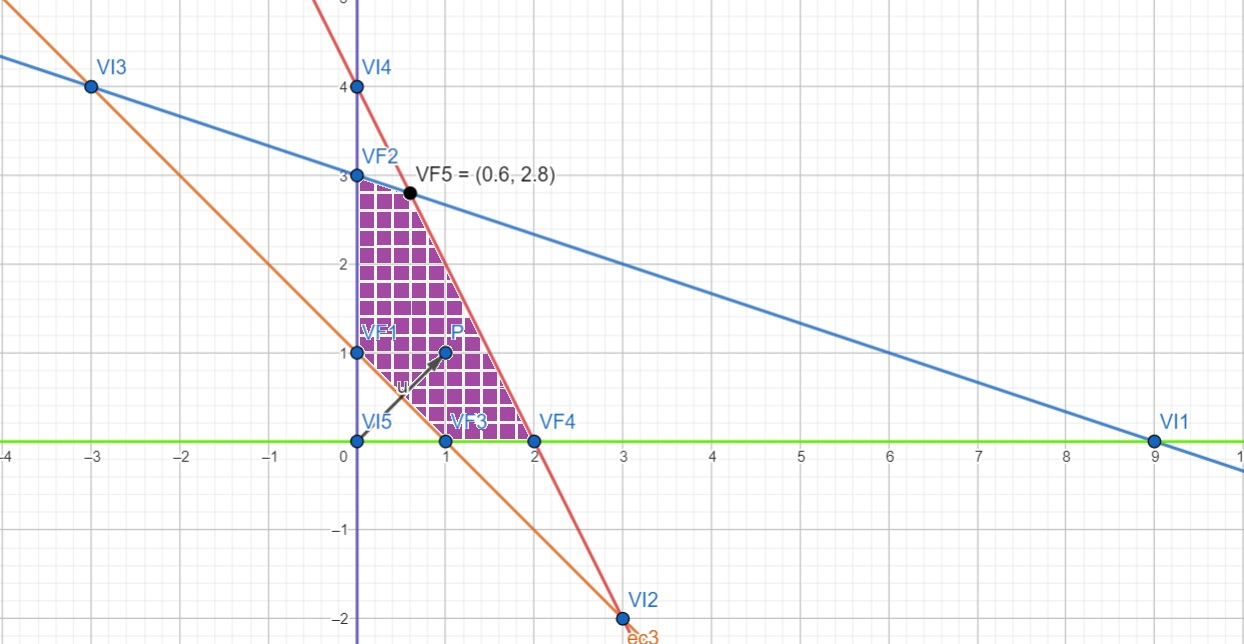
\includegraphics[width=1.1\textwidth]{grafico1.jpg}
			\caption{Gráfico pregunta 1}
			\label{fig:grafico}
		\end{figure}
		En el grafico y como se puede notar por la forma de la función objetivo, el vertice fáctible que cumple con ser la solución optima es $VF_5$ dado que alcanza el valor máximo siendo $3.4$.\\
		\newpage
		\begin{table}[ht]
			\centering
			\begin{tabular}{ccc}
				\hline
				\textbf{Vertice} & \textbf{Intersección} & \textbf{Coordenadas} \\
				\hline
				$VF_1$ & $R_3$ y $R_4$ & $(0, 1)$ \\
				$VF_2$ & $R_1$ y $R_4$ & $(0, 3)$\\
				$VF_3$ & $R_3$ y $R_5$ & $(1, 0)$ \\
				$VF_4$ & $R_2$ y $R_5$ & $(2, 0)$ \\
				$VF_5$ & $R_2$ y $R_1$  & $(0.6, 2.8)$ \\
				\hline
			\end{tabular}
			\caption{Vertices Factibles}
			\label{tab:vertices_factibles}
		\end{table}
		
		\begin{table}[ht]
			\centering
			\begin{tabular}{ccc}
				\hline
				\textbf{Vertice} & \textbf{Intersección} & \textbf{Coordenadas} \\
				\hline
				${VI}_1$ & $R_1$ y $R_5$ & $(9, 0)$ \\
				${VI}_2$ & $R_2$ y $R_3$ & $(3, -2)$\\
				${VI}_3$ & $R_1$ y $R_3$  & $(-3, 4)$\\
				${VI}_4$ & $R_4$ y $R_2$ & $(0, 4)$ \\
				${VI}_5$ & $R_4$ y $R_5$  & $(0, 5)$ \\
				\hline
			\end{tabular}
			\caption{Vertices Infactibles}
			\label{tab:vertices_infactibles}
		\end{table}

		
		\begin{table}[ht]
			\centering
			\begin{tabular}{cc}
				\hline
				\textbf{Restricción} & \textbf{Estado} \\
				\hline
				$R_1$ & Activa \\
				$R_2$ & Activa \\
				$R_3$ & Inactiva \\
				$R_4$ & Inactiva \\
				$R_5$ & Inactiva \\
				\hline
			\end{tabular}
			\caption{Restricciones activas e inactivas en $VF_5$} 
			\label{tab:tabla_ejemplo}
		\end{table}

		b) \\
		\vspace{0,5cm}
		\begin{center}
			\begin{align*}
				\text{P}) & \quad \min -x_1 - x_2 \\
				\text{s.a.} & \quad  R_1) \quad x_1 + 3x_2 \leq  9 \\
						   & \quad R_2) \quad 2x_1 + x_2 \leq  4 \\
						   & \quad R_3) \quad x_1 + x_2 \geq  1 \\
						   & \quad \quad x_1, x_2 \geq 0 \\
			\end{align*}
		\end{center}
		\begin{center}
			\begin{align*}
				\text{P} & \leftrightarrow \text{P} \\
			\end{align*}
		\end{center}

		\begin{center}
			\begin{align*}
				x_3) & \quad \text{Variable de holgura} \\
				x_4) & \quad \text{Variable de holgura} \\
				x_5) & \quad \text{Variable de exceso} \\
				\\
				\text{P}) & \quad \min -x_1 - x_2 \\
				\text{s.a.} & \quad  R_1) \quad x_1 + 3x_2 + x_3 = 9 \\
						   & \quad R_2) \quad 2x_1 + x_2 + x_4 = 4 \\
						   & \quad R_3) \quad x_1 + x_2 - x_5 = 1 \\
						   & \quad \quad x_1, x_2, x_3, x_4, x_5 \geq 0 \\
			\end{align*}
		\end{center}



		\vspace{0,5cm}
		c) \\
		
		\begin{center}
			\begin{align*}
				\text{P}) & \quad \min \quad x_6 + x_7 + x_8 \\
				\text{s.a.} & \quad  R_1) \quad x_1 + 3x_2 + x_3 + x_6 = 9 \\
						   & \quad R_2) \quad 2x_1 + x_2 + x_4 + x_7 = 4 \\
						   & \quad R_3) \quad x_1 + x_2 - x_5 + x_8 = 1 \\
						   & \quad \quad x_1, x_2, x_3, x_4, x_5, x_6, x_7, x_8 \geq 0 \\ 
			\end{align*}
		\end{center}

		Sea \( A \), la base \( B = \{6, 7, 8\} \), y \( X_B \):
		\begin{equation*}
			A =
			\left[
			\begin{array}{cccccccc}
			1 & 3 & 1 & 0 & 0 & 1 & 0  & 0  \\
			2 & 1 & 0 & 1 & 0 & 0 & 1 & 0 \\
			1 & 1 & 0 & 0 & -1 & 0 & 0 & 1  \\
			\end{array}
			\right], \quad
			B =
			\left\{ 6, 7, 8 \right\}, \quad
			X_B = I \cdot
			\left[
			\begin{array}{c}
			9 \\
			4 \\
			1 \\
			\end{array}
			\right] =
			\left[
			\begin{array}{c}
			9 \\
			4 \\
			1 \\
			\end{array}
			\right].
		\end{equation*}

		Entonces $Z = C_B^T X_B = 14$\\

		\vspace{0,5cm}
		Luego \(\bar{C}_n^\intercal\) se define como:
		\begin{equation*}
			\bar{C}_n^\intercal = 
			\begin{bmatrix}
				0 & 0 & 0
			\end{bmatrix} - 
			\begin{bmatrix}
				1 & 1 & 1
			\end{bmatrix} \cdot
			\begin{bmatrix}
				1 & 3 & 1 & 0 & 0  \\
				2 & 1 & 0 & 1 & 0  \\
				1 & 1 & 0 & 0 & -1  \\
			\end{bmatrix} = 
			\begin{bmatrix}
				-4 & -5 & -1 & -1 & 1
			\end{bmatrix}
		\end{equation*}
		\vspace{0,5cm}

		Por lo tanto haremos que $c_2$ entre a la base:

		\vspace{0,5cm}
		\begin{equation*}
			\begin{array}{c}
				u = A_b^-1 A_2 = [I]\begin{array}{c}
					3 \\
					1 \\
					1 \\
				\end{array}
			\end{array}
		\end{equation*}

		\[
		\delta^* = \min \left\{ \frac{9}{3}, \frac{4}{1}, \frac{1}{1} \right\} = 1
		\]
		\vspace{0,5cm}

		\[
		\begin{bmatrix} 9 \\ 4 \\ 1 \end{bmatrix} - 1 \cdot \begin{bmatrix} 3 \\ 1 \\ 1 \end{bmatrix} = \begin{bmatrix} 6 \\ 3 \\ 0 \end{bmatrix}
		\]

		El vector \(\tilde{x}_B\) se define como \([1, 6, 3]\) con \(B = \{2, 6, 7\}\), entonces \(x\) se obtiene como:
		\[
		x = (0, 1, 0, 0, 0, 6, 3)
		\]

		Entonces \( Z = C_B^T \cdot \tilde{x}_B = 9 < 14 \)

		Matriz \( A_b \):
		\[
		A_b = \begin{pmatrix}
		3 & 1 & 0 \\
		1 & 0 & 1 \\
		1 & 0 & 0 \\
		\end{pmatrix}
		\]

		Matriz inversa de \( A_b \):
		\[
		A_b^{-1} = \begin{pmatrix}
		0 & 0 & 1 \\
		1 & 0 & -3 \\
		0 & 1 & -1 \\
		\end{pmatrix}
		\]

		Luego \(\bar{C}_n^\intercal\) se define como:
		\begin{equation*}
			\bar{C}_n^\intercal = 
			\begin{bmatrix}
				0 & 0 & 0 & 0 & 1
			\end{bmatrix} - 
			\begin{bmatrix}
				0 & 1 & 1
			\end{bmatrix} \cdot
			\begin{bmatrix}
				0 & 0 & 1 \\
				1 & 0 & -3 \\
				0 & 1 & -1 \\
			\end{bmatrix} \cdot
			\begin{bmatrix}
				1 & 1 & 0 & 0 & 0  \\
				2 & 0 & 1 &  0 & 0  \\
				1 & 0 & 0 & -1 & 1  \\
			\end{bmatrix} = 
			\begin{bmatrix}
				1 & -1 & -1 & -4 & 5
			\end{bmatrix}
		\end{equation*}
	

		Por lo tanto haremos que $x_5$ entre a la base:
		Multiplicando la matriz \(\tilde{A}_5\) por el vector \([0, 0, -1]\):
		\[
		\begin{pmatrix}
		0 & 0 & 1 \\
		1 & 0 & -3 \\
		0 & 1 & -1 \\
		\end{pmatrix}
		\begin{pmatrix}
		0 \\
		0 \\
		-1 \\
		\end{pmatrix}
		=
		\begin{pmatrix}
		-1 \\
		3 \\
		2 \\
		\end{pmatrix}
		\]
		\[
			\delta^* = \min \left\{ \frac{1}{-1}, \frac{6}{3}, \frac{3}{1} \right\} = 2
		\]
		Entoces \(x_6\) sale:
		\[
		[1, 6, 3] - 2[-1, 3, 1] = [3, 0, 6]
		\]
		Con \(\tilde{x}_B = [3, 2, 1]\) y \(B = \{2, 5, 7\}\), el vector \(x\) se define como:
		\[
		x = (0, 3, 0, 0, 2)
		\]
		Matriz \( A_b \):
		\[
		A_b = \begin{pmatrix}
		3 & 0 & 0 \\
		1 & 0 & 1 \\
		1 & -1 & 0 \\
		\end{pmatrix}
		\]

		Matriz inversa de \( A_b \):
		\[
		A_b^{-1} = \begin{pmatrix}
		\frac{1}{3} & 0 & 0 \\
		\frac{1}{3} & 0 & -1 \\
		-\frac{1}{3} & 1 & 0 \\
		\end{pmatrix}
		\]
		Entonces \( Z = C_B^T \cdot \tilde{x}_B = 1 < 9 \)
		\newpage
		Luego \(\bar{C}_n^\intercal\) se define como:
		\begin{equation*}
			\bar{C}_n^\intercal = 
			\begin{bmatrix}
				0 & 0 & 0 & 1 & 1
			\end{bmatrix} - 
			\begin{bmatrix}
				0 & 0 & 1
			\end{bmatrix} \cdot
			\begin{bmatrix}
				\frac{1}{3} & 0 & 0 \\
				\frac{1}{3} & 0 & -1 \\
				-\frac{1}{3} & 1 & 0 \\
			\end{bmatrix} \cdot
			\begin{bmatrix}
				1 & 1 & 0 & 1 & 0  \\
				2 & 0 & 1 &  0 & 0  \\
				1 & 0 & 0 & 0 & 1  \\
			\end{bmatrix} = 
			\begin{bmatrix}
				-\frac{5}{3} & \frac{1}{3} & -1 & \frac{4}{3} & 1
			\end{bmatrix}
		\end{equation*}

		Por lo tanto, haremos que \(x_1\) entre a la base:
		Multiplicando la matriz \(\tilde{A}_1\) por el vector \([1, 2, 1]\):
		\[
		\begin{pmatrix}
		\frac{1}{3} & 0 & 0 \\
		\frac{1}{3} & 0 & -1 \\
		-\frac{1}{3} & 1 & 0 \\
		\end{pmatrix}
		\begin{pmatrix}
		1 \\
		2 \\
		1 \\
		\end{pmatrix}
		=
		\begin{pmatrix}
		\frac{1}{3} \\
		-\frac{2}{3} \\
		\frac{5}{3} \\
		\end{pmatrix}
		\]
		\[
			\delta^* = \min \left\{ \frac{3}{\frac{1}{3}}, \frac{2}{-\frac{2}{5}}, \frac{1}{\frac{5}{3}} \right\} = \frac{3}{5}
		\]
		\[
		[3, 2, 1] - \frac{3}{5}[\frac{4}{3}, -\frac{2}{3}, \frac{5}{3}] = [\frac{14}{5}, \frac{12}{5}, 0]
		\]
		Con \(x_b = \left[\frac{3}{5}, \frac{14}{5}, \frac{12}{5}\right]\) y \(B = \{1, 2, 5\}\), el vector \(x\) se define como:
		\[
		x = \left(\frac{3}{5}, \frac{14}{5}, 0, 0, \frac{12}{5}\right)
		\]
		Ahora \(x^* = \left(\frac{3}{5}, \frac{14}{5}, 0, 0, \frac{12}{5}, 0, 0, 0\right)\). Las variables artificiales son \(0\), entonces \(P\) es factible ya que el valor óptimo de \(F\) es \(0\).
		\vspace{0,5cm}
		
		d) \\
		\begin{center}
			\begin{align*}
				\text{P}) & \quad \min -x_1 - x_2 \\
				\text{s.a.} & \quad  R_1) \quad x_1 + 3x_2 + x_3 = 9 \\
						   & \quad R_2) \quad 2x_1 + x_2 + x_4 = 4 \\
						   & \quad R_3) \quad x_1 + x_2 - x_5 = 1 \\
						   & \quad  \quad x_1,x_2,x_3,x_4,_5x\geq 0\\
			\end{align*}
		\end{center}
		Con \(B = \{1, 2, 5\}\) entonces $A_b$ y $A_b^{-1}$ es:

		\(A_b =  \begin{pmatrix}
			1 & 3 & 0 \\
			2 & 1 & 0 \\
			1 & 1 & -1 \\
			\end{pmatrix}\)
			
			\(A_b^{-1} = \begin{pmatrix}
			\frac{-1}{5} & \frac{3}{5} & 0 \\
			\frac{2}{5} & \frac{-1}{5} & 0 \\
			-\frac{1}{5} & \frac{2}{5} & -1 \\
			\end{pmatrix}\)
			
			Multiplicando \(A_b^{-1}\) por el vector \([9, 4, 1]\) obtenemos \(\left[\frac{3}{5}, \frac{14}{5}, \frac{12}{5}\right]\).
			\vspace{0,5cm}

			Entonces \( Z = C_B^T \cdot \tilde{x}_B = \frac{-17}{5}\)

			Luego \(\bar{C}_n^\intercal\) se define como:
			\begin{equation*}
				\bar{C}_n^\intercal = 
				\begin{bmatrix}
					0 & 0 
				\end{bmatrix} - 
				\begin{bmatrix}
					-1 & -1 & 0
				\end{bmatrix} \cdot
				\begin{bmatrix}
					\frac{-1}{5} & \frac{3}{5} & 0 \\
					\frac{2}{5} & \frac{-1}{5} & 0 \\
					\frac{1}{5} & \frac{2}{5} & -1 \\
				\end{bmatrix} \cdot
				\begin{bmatrix}
					1 & 0 \\
					0 & 1   \\
					0 & 0  \\
				\end{bmatrix} = 
				\begin{bmatrix}
					\frac{1}{5} & \frac{2}{5}
				\end{bmatrix}
			\end{equation*}

			Como los costos reducidos son positivos, la solución actual es óptima tal que \(x^\star = \left(\frac{3}{5}, \frac{14}{5}, 0, 0, \frac{12}{5}\right)\)





	\end{flushleft}	
\end{document}	